\documentclass[11pt]{article}
\usepackage[margin=1in]{geometry}
\usepackage{amsmath}
\usepackage{graphicx}
\usepackage{float}
\usepackage{placeins}

\title{Meeting}

\begin{document}
\maketitle
\section{Overview}
  \begin{itemize}
    \item In our last meeting, I showed the results of our data shortening exercise, in which it appeared that the performance of our method seemed to get worse in when more data was available. I hypothesized that this was because the test set changed depending on the length. I changed the evaluation to make sure that the test set remained constant across different data lengths.  
    \item After changing this, we still observe the same phenomenon. However, both methods seem to be affected by it. 
    \item I also ran both methods on other midwestern states, our method outperformed Chen's in all other states and for all other lengths. However, there are times when neither method is better than no insurance. 
  \end{itemize}

\section{"Selling" the method}
  \begin{itemize}
    \item I think even without the multi-zone case this can be a significant contribution, at least to the index insurance literature. 
    \item We can think of our method as being somewhere in between Chantarat's method, which yielded explainable, but not optimized contracts, and Chen's method, which yields possibly optimal, but completely unexplainable contracts. 
    \item Our method yields contracts that are easily explainable, easily modified, and can accommodate constraints better than the two other methods. 
    \item Additionally, our method performs better in low data settings, which is better for the developing country context.
    \item If we include the multi-zone case, then it can also be an advantage of our method, of managing risk better in those scenarios. 
  \end{itemize}


\section{Results}
  \subsection{Illinois}
    As before, our method outperforms Chen's method when there is less data available. More specifically, our method outperforms Chen's when the data length is less than or equal to 40, which corresponds to data being available since 1970. However, most satellite data is available from 1980. Second, by looking at the cost plot we see that Chen's method seems to cost less. However, this is more from the model failing to recognize losses in the test set. The average payout in the training set tends to be higher than the average payout on the test set for Chen's model, even though average loss tends to be higher in the test set.  
    \subsubsection{Our definition of the premium}
    \begin{figure}[h]
        \centering
        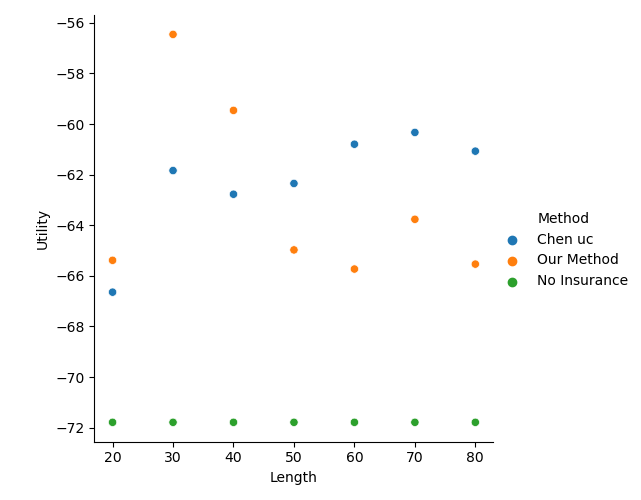
\includegraphics[width=0.6\textwidth]{../../../output/figures/Evaluation/Illinois_Utility_Length_ml1.png}
        \caption{Data shortening exercise using our definition of the premium. Here, Length is dataset length, or number of years of data available}
      \end{figure}
      \FloatBarrier

      \begin{figure}[h]
        \centering
        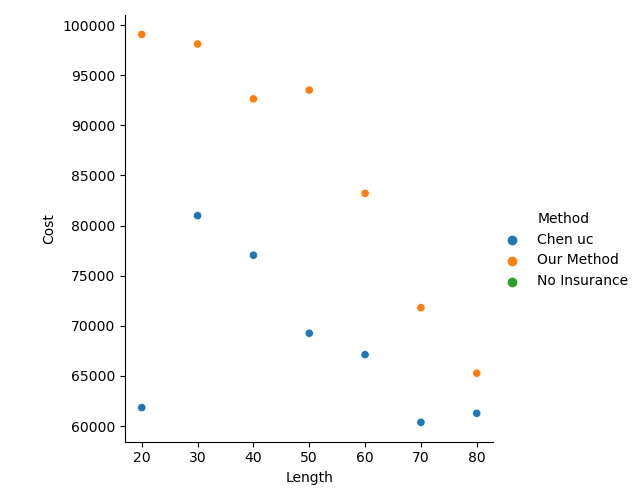
\includegraphics[width=0.6\textwidth]{../../../output/figures/Evaluation/Illinois_Cost_Length_ml1.png}
        \caption{Data shortening exercise using our definition of the premium. Here, Length is dataset length, or number of years of data available}
      \end{figure}
      \FloatBarrier

    \subsubsection{Their definition of the premium}
    Here, we observe a similar phenomenon as in the previous case, both the performance of both models tends to deteriorate as more data is added. Note that this doesn't contradict Chen's results, since in the full data case we get a similar utility improvement to what they reported in the paper ($13\%$ vs $14\%$).
    \begin{figure}[h]
        \centering
        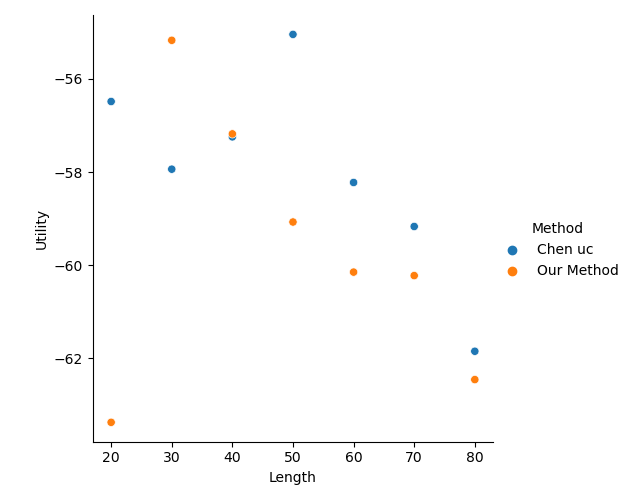
\includegraphics[width=0.6\textwidth]{../../../output/figures/Evaluation/Utility_length_ml1241.png}
        \caption{Data shortening exercise using our definition of the premium. Here, Length is dataset length, or number of years of data available}
      \end{figure}
      \FloatBarrier

      \begin{figure}[h]
        \centering
        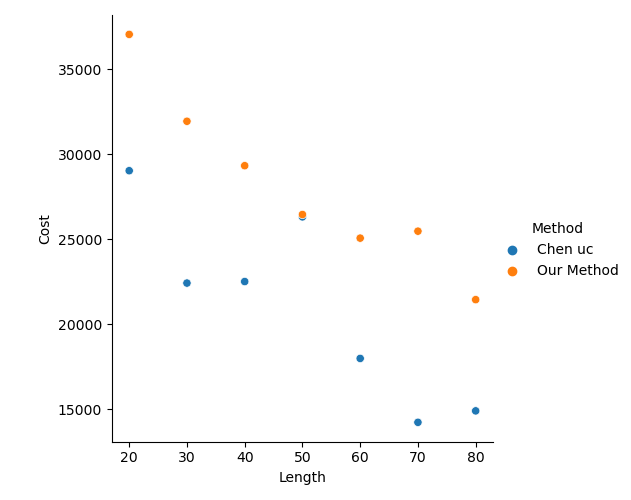
\includegraphics[width=0.6\textwidth]{../../../output/figures/Evaluation/Cost_length_ml1241.png}
        \caption{Data shortening exercise using our definition of the premium. Here, Length is dataset length, or number of years of data available}
      \end{figure}
      \FloatBarrier

  \subsection{Iowa}
    Here, our method outperforms Chen for all dataset lengths. Chen's method was much 
    \begin{figure}[h]
        \centering
        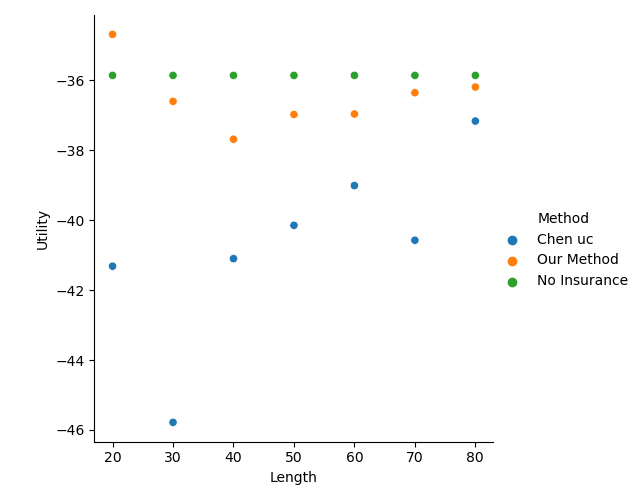
\includegraphics[width=0.6\textwidth]{../../../output/figures/Evaluation/Iowa_Utility_Length_ml1.png}
        \caption{Data shortening exercise using our definition of the premium. Here, Length is dataset length, or number of years of data available}
        \end{figure}
        \FloatBarrier

        \begin{figure}[h]
        \centering
        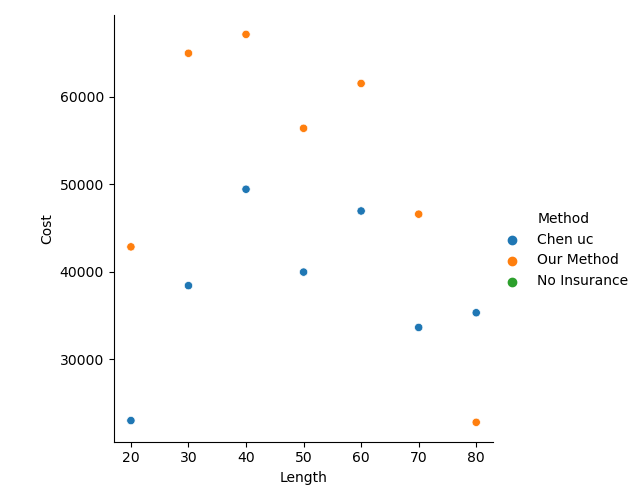
\includegraphics[width=0.6\textwidth]{../../../output/figures/Evaluation/Iowa_Cost_Length_ml1.png}
        \caption{Data shortening exercise using our definition of the premium. Here, Length is dataset length, or number of years of data available}
        \end{figure}
        \FloatBarrier

    \subsection{Indiana}
    \begin{figure}[h]
        \centering
        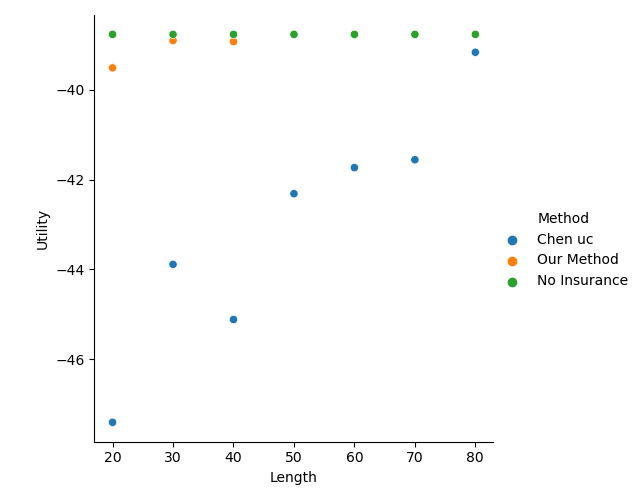
\includegraphics[width=0.6\textwidth]{../../../output/figures/Evaluation/Indiana_Utility_Length_ml1.png}
        \caption{Data shortening exercise using our definition of the premium. Here, Length is dataset length, or number of years of data available}
        \end{figure}
        \FloatBarrier

        \begin{figure}[h]
        \centering
        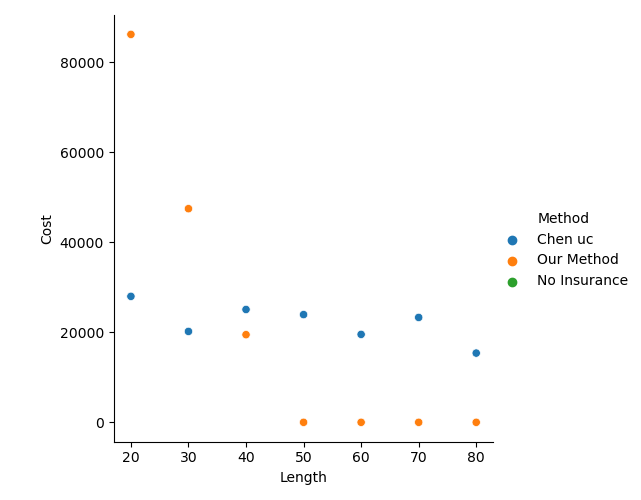
\includegraphics[width=0.6\textwidth]{../../../output/figures/Evaluation/Indiana_Cost_Length_ml1.png}
        \caption{Data shortening exercise using our definition of the premium. Here, Length is dataset length, or number of years of data available}
        \end{figure}
        \FloatBarrier

    \subsection{Missouri}
    \begin{figure}[h]
        \centering
        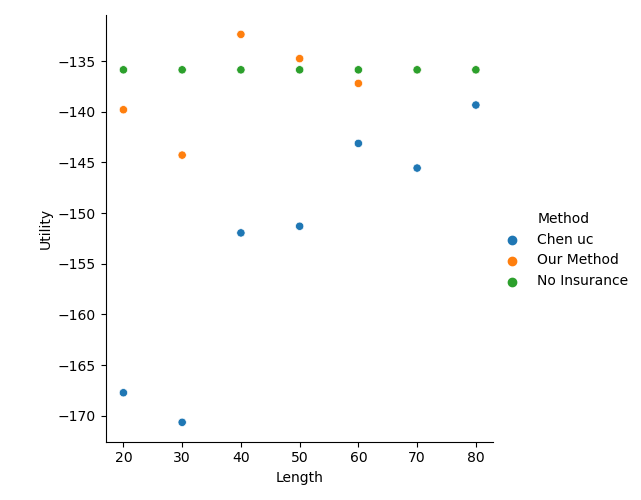
\includegraphics[width=0.6\textwidth]{../../../output/figures/Evaluation/Missouri_Utility_Length_ml1.png}
        \caption{Data shortening exercise using our definition of the premium. Here, Length is dataset length, or number of years of data available}
        \end{figure}
        \FloatBarrier

        \begin{figure}[h]
        \centering
        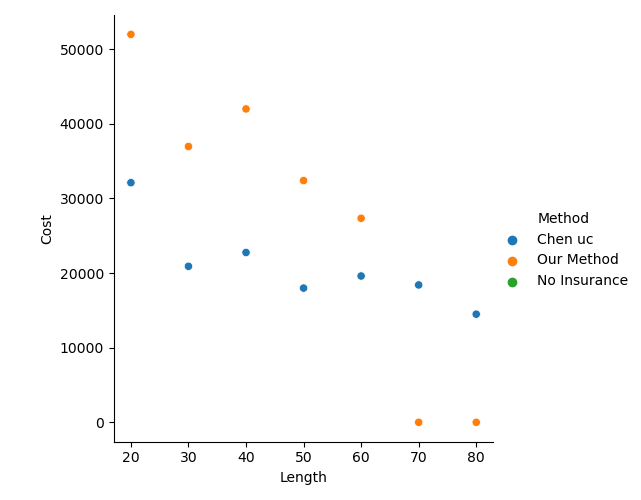
\includegraphics[width=0.6\textwidth]{../../../output/figures/Evaluation/Missouri_Cost_Length_ml1.png}
        \caption{Data shortening exercise using our definition of the premium. Here, Length is dataset length, or number of years of data available}
        \end{figure}
        \FloatBarrier

\section{Next Steps}
  There are a couple of things we can add, I'm listing them in order of how much I think they would add to the paper. 
\begin{itemize}
  \item \textbf{Multiple Zones:} This is almost done, it'll take another day to complete. 
  \item \textbf{Robustness to Misspecification:} I presented this at an econ workshop, and someone suggested that for the evaluation, I give each farmer a randomly chosen utility function, and that I compare how the two methods handle this. 
  \item \textbf{Descriptive Analysis:} We could create plots to illustrate the difference between the two methods: 
    \begin{enumerate}
      \item Plot of payouts vs losses
      \item Distribution of farmer utility/wealth
      \item Distribution of insurer costs
      \item Distribution of insurer profits
      \item Plot illustrating in what cases farmer's are worse off with insurance
    \end{enumerate}
\end{itemize}
\end{document}